\documentclass[tikz,border=5mm]{standalone}
\usepackage{tikz}
\usetikzlibrary{arrows.meta, positioning, fit, backgrounds}

\begin{document}
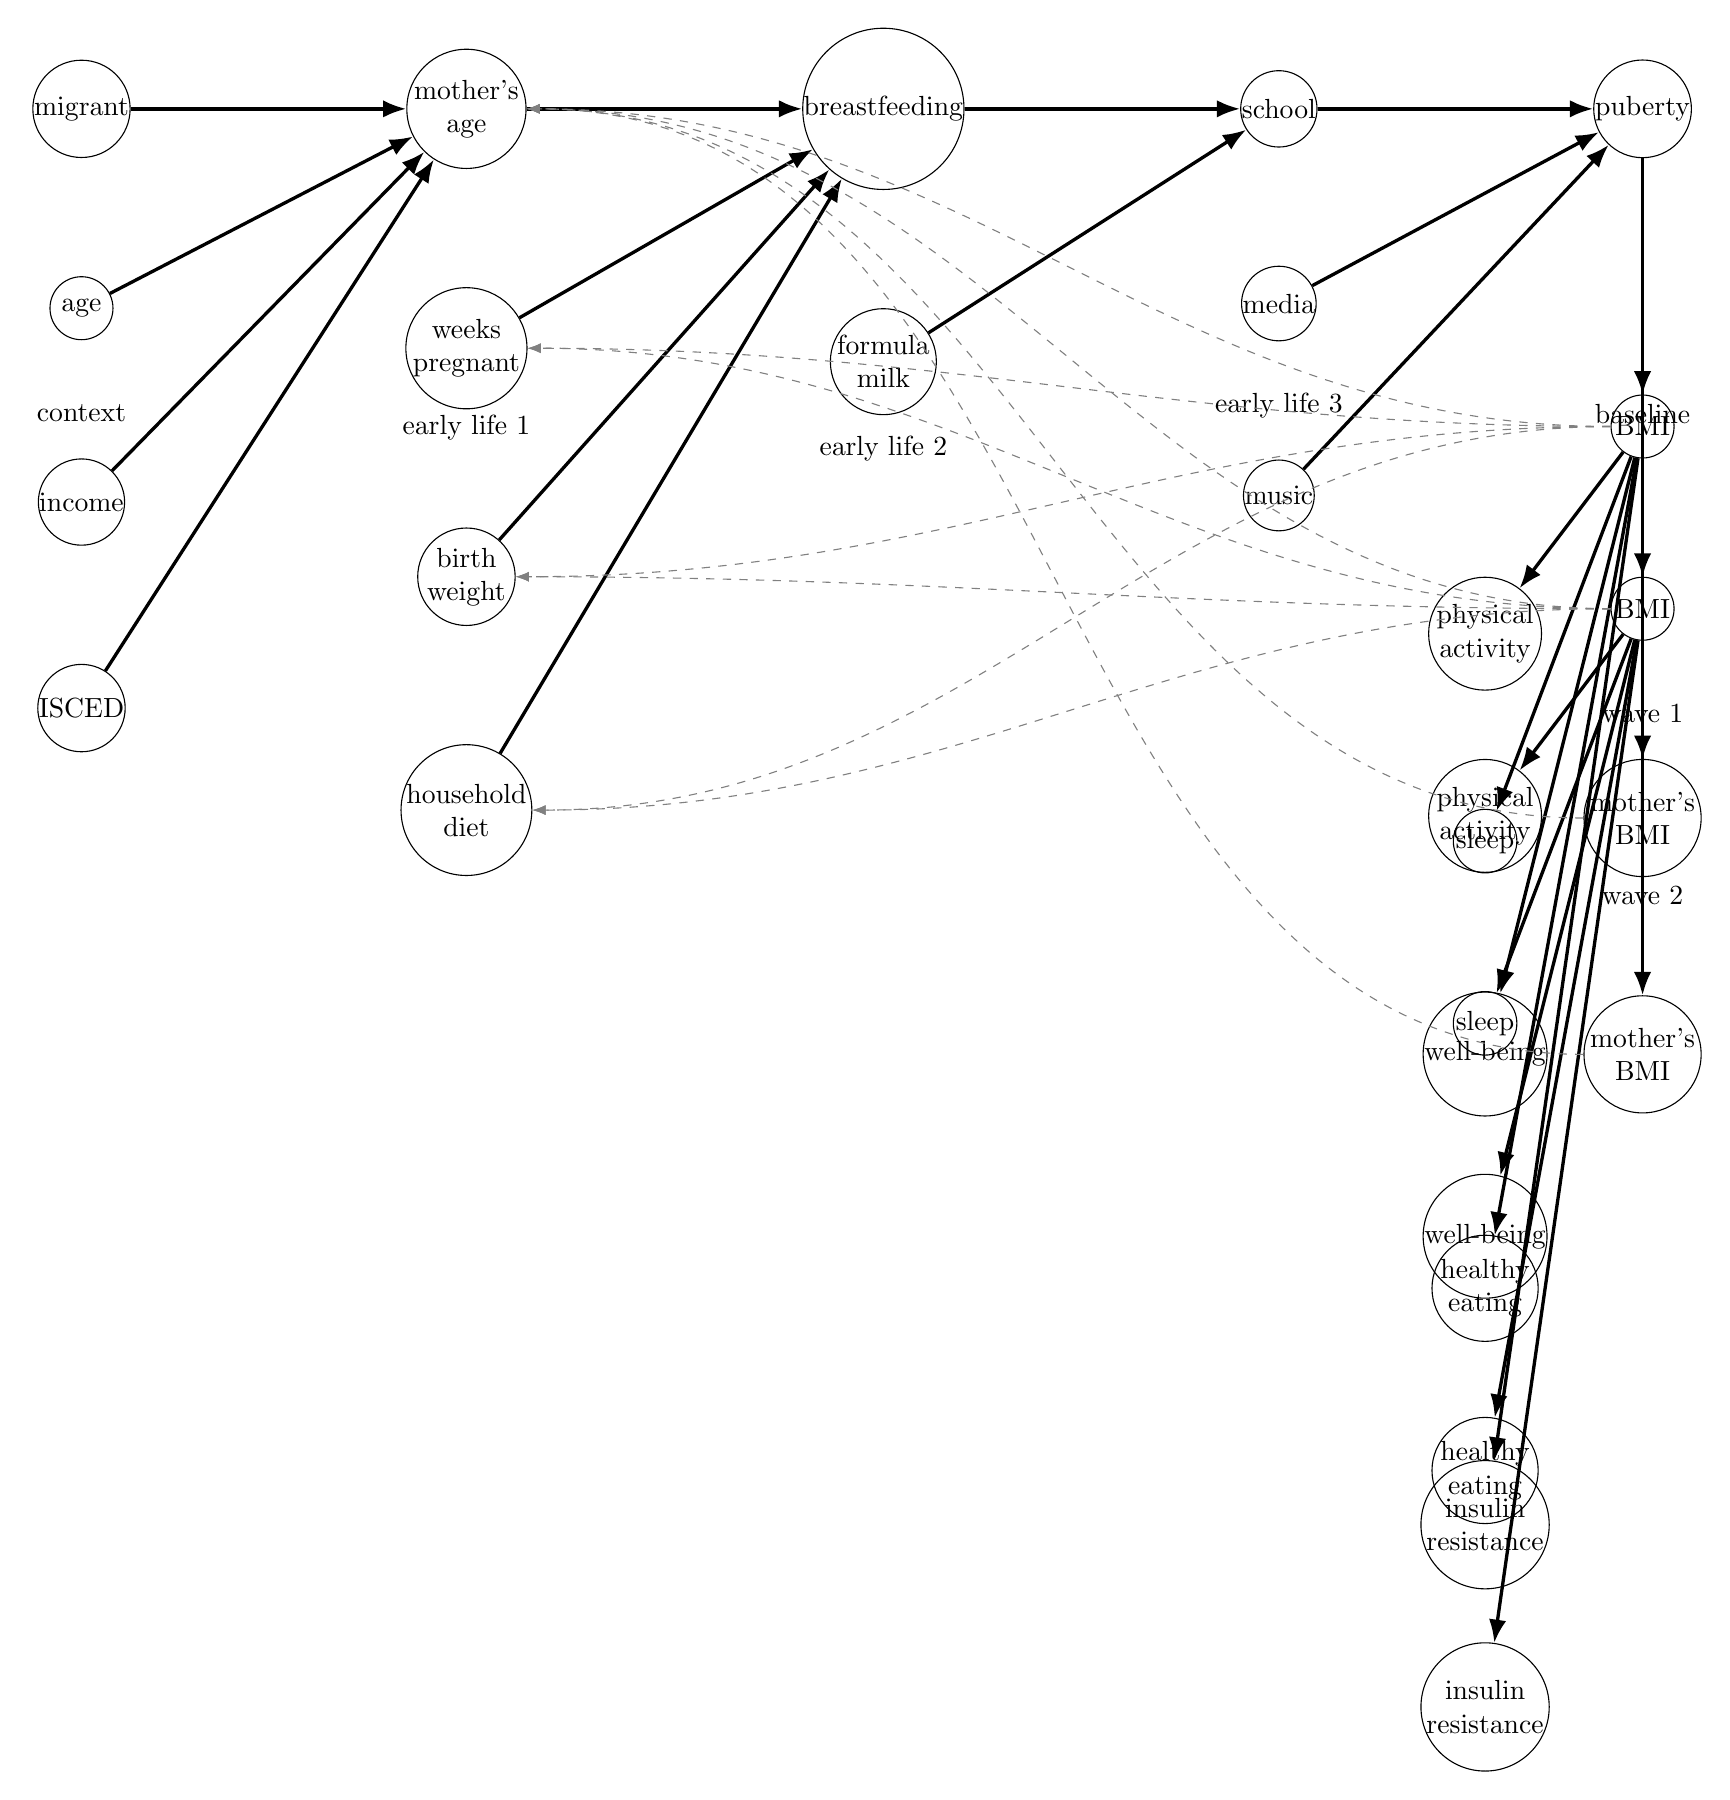
\begin{tikzpicture}[
    node distance=1.5cm,
    every node/.style={align=center},
    >=Latex,
    bold edge/.style={very thick, ->, black},
    dotted edge/.style={->, dashed, gray},
    mynode/.style={draw, circle, minimum size=8mm, inner sep=0pt},
]

% Define node styles and positions
\node[mynode] (migrant) {migrant};
\node[mynode, below=of migrant] (age) {age};
\node[mynode, below=of age] (income) {income};
\node[mynode, below=of income] (isced) {ISCED};

\node[mynode, right=of migrant, xshift=2cm] (mother_age) {mother's\\ age};
\node[mynode, below=of mother_age] (weeks_pregnant) {weeks\\ pregnant};
\node[mynode, below=of weeks_pregnant] (birth_weight) {birth\\ weight};
\node[mynode, below=of birth_weight] (household_diet) {household\\ diet};

\node[mynode, right=of mother_age, xshift=2cm] (breastfeeding) {breastfeeding};
\node[mynode, below=of breastfeeding] (formula_milk) {formula\\ milk};

\node[mynode, right=of breastfeeding, xshift=2cm] (school) {school};
\node[mynode, below=of school] (media) {media};
\node[mynode, below=of media] (music) {music};

\node[mynode, right=of school, xshift=2cm] (puberty) {puberty};

\node[mynode, below=of puberty, yshift=-1.5cm] (bmi_t_1) {BMI};
\node[mynode, below=of bmi_t_1] (bmi_t_2) {BMI};
\node[mynode, below=of bmi_t_2] (mother_bmi_t_1) {mother's\\ BMI};
\node[mynode, below=of mother_bmi_t_1] (mother_bmi_t_2) {mother's\\ BMI};

\node[mynode, below=of bmi_t_1, xshift=-2cm] (physical_activity_t_1) {physical\\ activity};
\node[mynode, below=of physical_activity_t_1] (sleep_t_1) {sleep};
\node[mynode, below=of sleep_t_1] (well-being_t_1) {well-being};
\node[mynode, below=of well-being_t_1] (healthy_eating_t_1) {healthy\\ eating};
\node[mynode, below=of healthy_eating_t_1] (insulin_resistance_t_1) {insulin\\ resistance};

\node[mynode, below=of bmi_t_2, xshift=-2cm] (physical_activity_t_2) {physical\\ activity};
\node[mynode, below=of physical_activity_t_2] (sleep_t_2) {sleep};
\node[mynode, below=of sleep_t_2] (well-being_t_2) {well-being};
\node[mynode, below=of well-being_t_2] (healthy_eating_t_2) {healthy\\ eating};
\node[mynode, below=of healthy_eating_t_2] (insulin_resistance_t_2) {insulin\\ resistance};

% Add column labels
\node[below=of migrant, yshift=-1.5cm] (context_label) {context};
\node[below=of mother_age, yshift=-1.5cm] (early_life1_label) {early life 1};
\node[below=of breastfeeding, yshift=-1.5cm] (early_life2_label) {early life 2};
\node[below=of school, yshift=-1.5cm] (early_life3_label) {early life 3};
\node[below=of puberty, yshift=-1.5cm] (baseline_label) {baseline};
\node[below=of bmi_t_1, yshift=-1.5cm] (wave1_label) {wave 1};
\node[below=of bmi_t_2, yshift=-1.5cm] (wave2_label) {wave 2};

% Draw edges
% Bold edges: within-time and across-time plausible edges
\draw[bold edge] (migrant) -- (mother_age);
\draw[bold edge] (age) -- (mother_age);
\draw[bold edge] (income) -- (mother_age);
\draw[bold edge] (isced) -- (mother_age);

\draw[bold edge] (mother_age) -- (breastfeeding);
\draw[bold edge] (weeks_pregnant) -- (breastfeeding);
\draw[bold edge] (birth_weight) -- (breastfeeding);
\draw[bold edge] (household_diet) -- (breastfeeding);

\draw[bold edge] (breastfeeding) -- (school);
\draw[bold edge] (formula_milk) -- (school);

\draw[bold edge] (school) -- (puberty);
\draw[bold edge] (media) -- (puberty);
\draw[bold edge] (music) -- (puberty);

\draw[bold edge] (puberty) -- (bmi_t_1);
\draw[bold edge] (puberty) -- (bmi_t_2);
\draw[bold edge] (puberty) -- (mother_bmi_t_1);
\draw[bold edge] (puberty) -- (mother_bmi_t_2);

\draw[bold edge] (bmi_t_1) -- (physical_activity_t_1);
\draw[bold edge] (bmi_t_1) -- (sleep_t_1);
\draw[bold edge] (bmi_t_1) -- (well-being_t_1);
\draw[bold edge] (bmi_t_1) -- (healthy_eating_t_1);
\draw[bold edge] (bmi_t_1) -- (insulin_resistance_t_1);

\draw[bold edge] (bmi_t_2) -- (physical_activity_t_2);
\draw[bold edge] (bmi_t_2) -- (sleep_t_2);
\draw[bold edge] (bmi_t_2) -- (well-being_t_2);
\draw[bold edge] (bmi_t_2) -- (healthy_eating_t_2);
\draw[bold edge] (bmi_t_2) -- (insulin_resistance_t_2);

% Dotted edges: implausible edges violating time ordering
\draw[dotted edge] (bmi_t_1) to[out=180,in=0] (mother_age);
\draw[dotted edge] (bmi_t_1) to[out=180,in=0] (weeks_pregnant);
\draw[dotted edge] (bmi_t_1) to[out=180,in=0] (birth_weight);
\draw[dotted edge] (bmi_t_1) to[out=180,in=0] (household_diet);

\draw[dotted edge] (bmi_t_2) to[out=180,in=0] (mother_age);
\draw[dotted edge] (bmi_t_2) to[out=180,in=0] (weeks_pregnant);
\draw[dotted edge] (bmi_t_2) to[out=180,in=0] (birth_weight);
\draw[dotted edge] (bmi_t_2) to[out=180,in=0] (household_diet);

\draw[dotted edge] (mother_bmi_t_1) to[out=180,in=0] (mother_age);
\draw[dotted edge] (mother_bmi_t_2) to[out=180,in=0] (mother_age);

\end{tikzpicture}
\end{document}